\section{Alcance}\label{sec:alcance}

El alcance de este proyecto incluye el trabajo necesario para diseñar,
implementar y documentar un framework de modelado y desarrollo de simulación de
sistemas dinámicos discretos basados en eventos. Dicho framework se dividirá en
tres módulos principales:
\begin{itemize}
    \item Lenguaje: Un lenguaje de modelado específico pensado para ser usado
    por usuarios que no tengan mucha experiencia en programación. Se hará uso de
    las herramientas de desarrollo de compiladores Flex y Bison para generar un
    transpilador que traduzca ficheros de este lenguaje a código Python. A
    través de él se plantea:
    \begin{itemize}
        \item Permitir la rápida implementación de este tipo de modelos a través
        de grafos de sucesos.
        \item Permitir que el programador del lenguaje se encargue sólo de
        realizar las implementaciones pertinentes al sistema de simulación que
        desee desarrollar:
        \begin{itemize}
            \item Especificación de las variables globales, variables de
            entrada, contadores estadísticos y medidas de rendimiento propias
            del modelo.
            \item Inclusión de eventos adicionales y sus acciones
            correspondientes.
            \item Creación y eliminación de eventos en función de tiempo y
            condiciones lógicas.
            \item Inclusión de código adicional escrito directamente en Python
            en caso de ser necesario.\urgent{Cambiar redacción}
        \end{itemize}
    \end{itemize}
    \item Núcleo: Una serie de módulos que implementarán un microframework de
    simulación de este tipo de sistemas en específico para Python, pensado para
    ser usado por programadores y para acotar la traducción del nuevo lenguaje.
    A través de él se plantea:
    \begin{itemize}
        \item Permitir que la traducción del lenguaje incluya dentro del fichero
        generado las estructuras de datos, funciones y procedimientos que tienen
        en común todos los sistemas dinámicos discretos:
        \begin{itemize}
            \item Generadores de datos aleatorios para distintos tipos de
            distribuciones.
            \item Reloj y temporizador de simulación para ejecutar los eventos.
            \item Estructura de datos para almacenar los sucesos según deben
            ocurrir en el tiempo.
            \item Las respectivas implementaciones mínimas de los dos eventos
            que siempre formarán parte de todos los modelos: “Inicio” y “Fin”.
            \item Generador de informes final que se ejecutará al finalizar la
            simulación y mostrará los resultados que se deseaban estudiar con
            ésta.
        \end{itemize}
    \end{itemize}
    \item CLI: Una interfaz de comandos por terminal que se usará para
    gestionar, configurar y ejecutar los proyectos desarrollados con este
    framework.
\end{itemize}

\subsection{Objetivos}

\subsubsection{Objetivo general}
Generar un lenguaje de modelado de simulación de sistemas dinámicos discretos
basados en eventos junto con un transpilador que lo traduzca a Python, un
microframework para acotar la traducción y un CLI para gestionar proyectos
desarrollados con este producto.

\subsubsection{Objetivos específicos}
\begin{enumerate}
    \item Diseñar un nuevo lenguaje de modelado y simulación de sistemas
    dinámicos discretos basados en eventos usando las herramientas de desarrollo
    de procesadores de lenguaje Flex y Bison.
    \item Diseñar, implementar y verificar una serie de módulos y
    funcionalidades realizadas en Python con el fin de generar un microframework
    para simular estos mismos sistemas.
    \item Implementar y verificar un transpilador que traduzca el lenguaje del
    producto a Python usando las características del objetivo anterior.
    \item Diseñar, implementar y verificar una serie de operaciones accesibles
    desde una CLI de cara a ser usadas para la gestión, configuración y
    ejecución parametrizada de simulaciones realizadas con el producto.
    \item Implementar distintas técnicas de análisis de salidas, experimentación
    y optimización de modelos dentro del núcleo del framework.
    \item Desarrollar un manual de usuario que contendrá toda la documentación
    necesaria para hacer uso del framework.
\end{enumerate}

\subsection{Requisitos}
El requisito base principal del proyecto consiste en cumplir con un tiempo de
dedicación total máximo de 300 horas. Sin embargo, se pueden listar otros
requisitos específicos:

\subsubsection{Caracterización de la memoria}
Debe ser bien citado y referenciado para evitar el plagio
Se debe utilizar una metodología de citas.
Apartado de calidad

\subsubsection{Caracterización del framework}
Un lenguaje verificado que no pete a la primera
El resultado son métricas en un dataframe (o varios si harás lo de validación)
Cumplir con la línea base de calidad definida en el apartado (...)

\subsubsection{Caracterización del manual}
Utilizar referencias a recursos ajenas

\subsubsection{Licencia del producto}

\subsection{Entregables}

\begin{itemize}
    \item Memoria: \change{Relacionados con el objeto de proyecto en sí}
    \item Framework:\change{Relacionados con el objeto de proyecto en sí}
    \item Manual: \change{Relacionados con el objeto de proyecto en sí}
    \item Planificación: \change{Relacionados con la Planificación y Gestión del
    Proyecto}
    \item Seguimiento y Control: \change{Relacionados con la Planificación y Gestión del
    Proyecto}
    \item Actas: \change{Relacionados con la Planificación y Gestión del
    Proyecto}
\end{itemize}

\subsection{Exclusiones}

Mi proyecto devolverá los datos en un sólo formato, no devolveré más tipos de
ficheros para darle gusto al usuario.

\subsection{Supuestos}

\urgent[inline]{}

\subsection{EDT}

\begin{figure}[H]
    \centering
    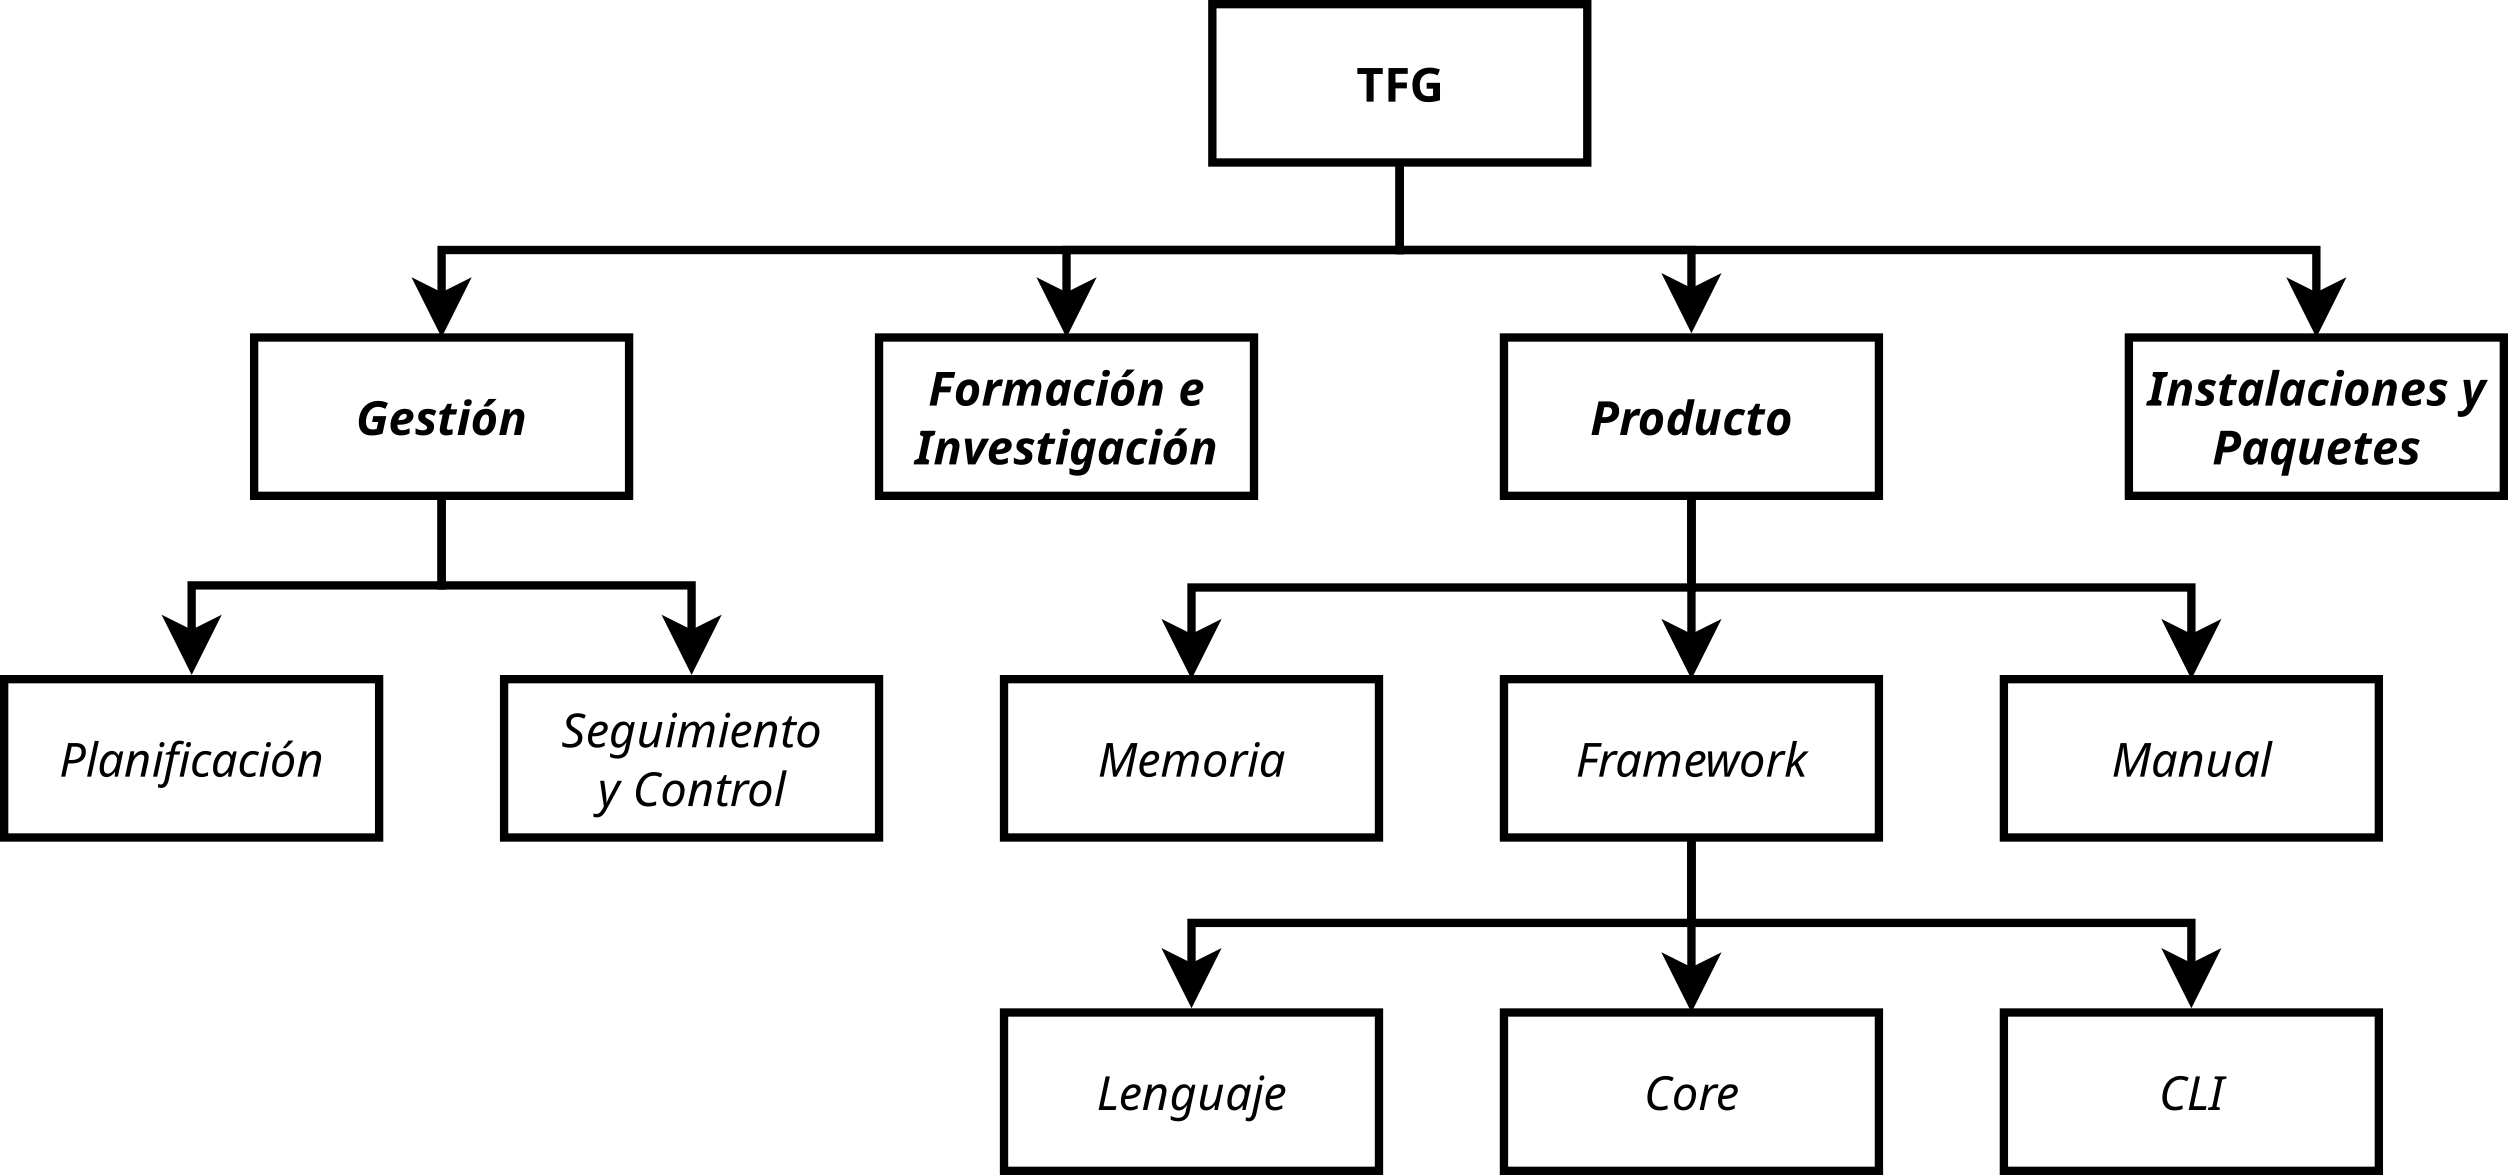
\includegraphics[width=\textwidth]{5-Cuerpo/Chapter1/EDT.png}
    \caption{Esquema de Descomposición de Trabajo del Proyecto}
    \label{fig:EDT}
\end{figure}